\documentclass[3p]{elsarticle}

\usepackage[utf8]{inputenc}
\usepackage[T1]{fontenc}
\usepackage{lmodern}
\usepackage{amsmath,amssymb,amsthm,mathtools}
\usepackage{booktabs}
\usepackage[shortlabels]{enumitem}
\usepackage{xcolor}
\usepackage[hidelinks]{hyperref}
\usepackage[capitalise,noabbrev]{cleveref}
\pdfstringdefDisableCommands{\def\corref#1{}}
\usepackage{microtype}
\usepackage{url}
\usepackage{tikz}
%% TikZ definitions for the drawings of Figures 1-7 (state colours as in the space-time diagrams).
%% State colours are those of the space-time diagrams (figures.py).
\usetikzlibrary{shapes.geometric,shapes.callouts,arrows.meta,decorations.pathmorphing,calc,patterns}
\definecolor{stL}{HTML}{E2DFD6}
\definecolor{stG}{HTML}{2A78D6}
\definecolor{stA}{HTML}{EB6834}
\definecolor{stB}{HTML}{1BAF7A}
\definecolor{stF}{HTML}{0B0B0B}
\definecolor{ink}{HTML}{0B0B0B}
\definecolor{ink2}{HTML}{52514E}
\definecolor{skin}{HTML}{F1C9A5}
\definecolor{brick}{HTML}{B5523B}
\definecolor{paper}{HTML}{F4F3F0}
\definecolor{agree}{HTML}{DCE9F8}
\definecolor{refl}{HTML}{FBE3D6}
\definecolor{flash}{HTML}{FFD23F}

%% \soldier{x}{y}{state}{face}: a soldier standing at (x,y) (feet), tunic in the
%% colour of the state, the state letter on the tunic; face = sleep|awake|shout|fire.
\newcommand{\soldier}[4]{%
  \edef\sdState{#3}\edef\sdFace{#4}\edef\sdCol{st#3}%
  \ifdefstring{\sdState}{L}{\def\sdText{ink}}{\def\sdText{white}}%
  \begin{scope}[shift={(#1,#2)}]
    \draw[ink,line width=1pt,line cap=round] (-0.06,0.40) -- (-0.09,0.06);
    \draw[ink,line width=1pt,line cap=round] (0.06,0.40) -- (0.09,0.06);
    \fill[ink] (-0.16,0) rectangle (-0.04,0.06);
    \fill[ink] (0.04,0) rectangle (0.16,0.06);
    \ifdefstring{\sdFace}{fire}{%
      \draw[brick!60!black,line width=1.6pt,line cap=round] (-0.02,0.50) -- (0.30,1.30);
      \node[star,star points=10,star point ratio=2.1,fill=flash,draw=stA,line width=0.4pt,
            inner sep=0pt,minimum size=0.36cm] at (0.33,1.40) {};
    }{}%
    \filldraw[fill=\sdCol,draw=ink,line width=0.5pt,rounded corners=1.2pt]
      (-0.16,0.38) rectangle (0.16,0.84);
    \ifdefstring{\sdFace}{fire}{%
      \draw[ink,line width=1pt,line cap=round] (-0.14,0.78) -- (0.05,0.66) -- (0.14,0.86);
    }{%
      \draw[ink,line width=1pt,line cap=round] (-0.19,0.80) -- (-0.21,0.46);
      \draw[ink,line width=1pt,line cap=round] (0.19,0.80) -- (0.21,0.46);
    }%
    \node[font=\sffamily\bfseries\scriptsize,text=\sdText] at (0,0.61) {\sdState};
    \filldraw[fill=skin,draw=ink,line width=0.5pt] (0,1.00) circle (0.13);
    \filldraw[fill=ink!85,draw=ink,line width=0.4pt]
      (-0.145,1.07) -- (0.145,1.07) -- (0.11,1.19) -- (-0.11,1.19) -- cycle;
    \ifdefstring{\sdState}{G}{\node[star,star points=5,fill=flash,inner sep=0pt,minimum size=0.11cm] at (0,1.13) {};}{}%
    \ifdefstring{\sdFace}{sleep}{%
      \draw[ink,line width=0.45pt] (-0.075,1.005) arc (180:360:0.028);
      \draw[ink,line width=0.45pt] (0.019,1.005) arc (180:360:0.028);
    }{%
      \fill[ink] (-0.047,1.0) circle (0.016);
      \fill[ink] (0.047,1.0) circle (0.016);
    }%
    \ifdefstring{\sdFace}{shout}{\fill[ink] (0,0.935) ellipse (0.03 and 0.022);}{}%
    \ifdefstring{\sdFace}{fire}{\fill[ink] (0,0.935) ellipse (0.035 and 0.025);}{}%
    \ifdefstring{\sdFace}{awake}{\draw[ink,line width=0.4pt] (-0.03,0.94) -- (0.03,0.94);}{}%
  \end{scope}}

%% \zzz{x}{y}: sleeping marks
\newcommand{\zzz}[2]{%
  \node[font=\sffamily\bfseries\tiny,text=ink2] at (#1+0.20,#2+1.22) {z};
  \node[font=\sffamily\bfseries\scriptsize,text=ink2] at (#1+0.30,#2+1.37) {z};}

%% \brickwall{x}{y}{height}: the border, drawn as a brick wall 0.24 wide
\newcommand{\brickwall}[3]{%
  \begin{scope}[shift={(#1,#2)}]
    \fill[brick] (0,0) rectangle (0.24,#3);
    \foreach \yy in {0.15,0.30,...,#3} {\draw[white,line width=0.5pt] (0,\yy) -- (0.24,\yy);}
    \node[font=\small,text=ink2] at (0.12,#3+0.18) {$\ast$};
  \end{scope}}

%% \stone{k}{x}{colour}{verdict}{references}: a stepping stone of the state-count scoreboard
\newcommand{\stone}[5]{%
  \filldraw[fill=#3,draw=ink,line width=0.5pt] (#2,0) circle (0.3);
  \node[font=\small\bfseries,text=white] at (#2,0) {#1};
  \node[font=\scriptsize,anchor=north] at (#2,-0.36) {#4};
  \node[font=\scriptsize,anchor=north,align=center,text=ink2] at (#2,-0.66) {#5};}


\newtheorem{theorem}{Theorem}[section]
\newtheorem{lemma}[theorem]{Lemma}
\newtheorem{proposition}[theorem]{Proposition}
\newtheorem{corollary}[theorem]{Corollary}
\theoremstyle{remark}
\newtheorem{remark}[theorem]{Remark}

\begin{document}

\begin{frontmatter}

\title{Two necessary conditions on minimal-time solutions\\
of the firing squad problem}

\author[tjc]{Kia Keng Giam\corref{cor1}}
\ead{giamkiakeng@gmail.com}
\cortext[cor1]{Corresponding author.}
\author[hci]{Beichen Sun}
\author[hci]{Yaoqi Zhao}

\affiliation[tjc]{organization={Temasek Junior College},
            country={Singapore}}
\affiliation[hci]{organization={Hwa Chong Institution},
            country={Singapore}}

\begin{abstract}
We prove two necessary conditions on the space-time diagram of every
minimal-time solution of the firing squad synchronization problem, whatever
its number of states. Every line agrees with the infinite half-line until the
echo of its right end returns, and the rest of the line is a function of two
anti-diagonals of the half-line. First, a pumping argument at the right end
shows that the non-periodic part of the half-line reaches the line $i=t/3$
behind the front. Second, near the left border the reflected part of the line
acts as a finite-state transducer on the half-line and cannot time the firing
along long periodic stretches; hence the half-line is not periodic in any wedge
at the left border, and it is never eventually regular. Both conditions can be
checked on computed half-lines. With computer assistance, including
LRAT-certified unsatisfiability proofs, we use them to show that every
five-state minimal-time solution uses at least $15$ distinct neighbourhoods on
its half-line below the anti-diagonal $t+i=78$, to re-prove with a certificate
that four states do not suffice, and to confirm a conditional five-state result
claimed by Balzer in 1967. A five-state rule that synchronizes all lines of
length at most $14$ bounds what refutations of this kind can achieve.
\end{abstract}

\begin{keyword}
firing squad synchronization problem \sep cellular automata \sep state
complexity \sep minimal time \sep pumping lemma \sep proof certificates
\end{keyword}

\end{frontmatter}

%% ---------------------------------------------------------------------
\section{Introduction}\label{sec:intro}

The firing squad synchronization problem, posed by Myhill in 1957 and
popularised by Moore \cite{Moore64}, asks for a finite automaton that, placed
in every cell of a line of arbitrary length $n$ and started with all cells
quiescent except a \emph{general} at one end, drives all cells into a firing
state for the first time at the same instant. Goto \cite{Goto62} and Waksman
\cite{Waksman66} solved it in time $2n-2$, which is optimal. This note proves
two necessary conditions on every minimal-time solution, whatever its number
of states. In the frame of the front the cells at a fixed depth behind the
front become periodic in time, but along infinitely many depths the
non-periodic part reaches the line $i=t/3$ (\cref{thm:third}). The half-line
is not periodic in time and space on any wedge at the left border
(\cref{thm:left}); hence it is never eventually regular, i.e.\ it never
consists of finitely many periodic regions separated by signals of rational
speeds (\cref{cor:regular}).

The least number of states of a minimal-time solution is a benchmark question
\cite{Umeo09,Correa17}: Waksman used $16$ states, Balzer $8$ \cite{Balzer67},
Gerken $7$ \cite{Gerken87} and Mazoyer $6$ \cite{Mazoyer87}. Balzer reported a
computer search excluding four states \cite{Balzer67}; Yun\`es \cite{Yunes93}
repeated it and observed that the lines of lengths $2,\dots,9$ suffice, and
Sanders \cite{Sanders94} found Balzer's backtracking incomplete and confirmed
the result with a corrected search. Whether five states suffice has been open
since 1987. As there are finitely many $k$-state rules, $k$-state minimal-time
solutions do not exist if and only if for some $N$ no $k$-state rule
synchronizes all lines of lengths $2,\dots,N$ in minimal time, so a negative
answer may consist of finitely many necessary conditions. (Existence is
different: the set of minimal-time solutions is not recursively enumerable
\cite{Mazoyer96}.)

Our conditions rest on an elementary decomposition (\cref{sec:prelim}): until
the echo of its right border returns, the line of length $n$ behaves like the
infinite half-line, so a solution consists of one half-line diagram $C_\infty$
and, for each $n$, a triangle $R_n$ that is a function of two anti-diagonals of
$C_\infty$ (\cref{lem:determinacy}). The right end of $R_n$ must fire at time
$2n-2$, so the inputs of the triangles of two lengths must differ on an
explicit cone (\cref{lem:pumping}); this gives \cref{thm:third}. At the left
end, $R_n$ is computed by a band of anti-diagonals that acts as a finite-state
transducer on $C_\infty$ (\cref{lem:left}, with the explicit bound
$(k-1)^{2s}\ell$); this gives \cref{thm:left}. The two conditions complement
each other: the half-line of two five-state rules attains the bound of
\cref{thm:third} with equality but violates \cref{lem:left}
(\cref{rem:optimal,cor:germ12}). \Cref{sec:computations} applies them, with
computer assistance, to four and five states: a certificate for the four-state
bound (\cref{thm:four}), a five-state rule for all lengths up to $14$
(\cref{prop:chaotic}), the bound $c_{78}\ge15$ on the complexity of the
half-line of every five-state solution (\cref{prop:germs}), and Balzer's
conditional result (\cref{prop:balzer}).

\paragraph{Related work} Indistinguishability arguments, in which two
situations that a solution cannot tell apart force some cell to fire too
early, exclude minimal-time solutions with one-way channels (Mazoyer
\cite[Prop.~2]{Mazoyer96} compares the lines of lengths $2$, $3$ and $4$) and,
through a repetition of a pair of states forced by the pigeonhole principle,
for variants with sub-generals and some geometric configurations
\cite{YamashitaEtAl14,Kobayashi19} (we follow the description in
\cite{Kobayashi19}). Our pumping lemma applies this mechanism to the original
problem and to all lengths, where it constrains solutions instead of excluding
them. The eventual periodicity behind the front used in \cref{thm:third} is
classical and underlies the work of Mazoyer and Terrier on signals
\cite{MazoyerTerrier94,MazoyerTerrier99}. Lower bounds are known for restricted
classes: no three-state solution and no four-state symmetric minimal-time
solution exist for rings \cite{BerthiaumeEtAl04}, and Settle's thesis
\cite{Settle99}, as described in \cite{Correa17}, excludes four- and five-state
solutions under additional constraints. Solutions with at most five states
exist for restricted families of lengths such as the powers of two, some of
them in non-minimal time \cite{UmeoYanagihara07,Yunes08}. Propositional
encodings of cellular automata have been used for reachability questions
\cite{DAntonioDelzanno04}. We are not aware of statements equivalent to
\cref{thm:third,thm:left} or \cref{cor:regular} in the literature.

%% ---------------------------------------------------------------------
\section{Lines and the half-line}\label{sec:prelim}

Let $S$ be a finite set of \emph{states} containing three pairwise distinct
states, the quiescent state $\mathsf L$, the general $\mathsf G$ and the firing
state $\mathsf F$; the \emph{working} states are $W:=S\setminus\{\mathsf F\}$,
the \emph{auxiliary} states are $W\setminus\{\mathsf L,\mathsf G\}$, and
$\ast\notin S$ denotes the border. A \emph{rule} is a map
$\delta:(W\cup\{\ast\})\times W\times(W\cup\{\ast\})\to S$ with
\begin{equation}\label{eq:quiescence}
\delta(\mathsf L,\mathsf L,\mathsf L)=\delta(\mathsf L,\mathsf L,\ast)=\mathsf L .
\end{equation}
The \emph{line of length $n$} is $C_n:\mathbb N\times\{1,\dots,n\}\to S$ with
$C_n(0,1)=\mathsf G$, $C_n(0,i)=\mathsf L$ for $i\ge2$ and
$C_n(t+1,i)=\delta(C_n(t,i-1),C_n(t,i),C_n(t,i+1))$, where
$C_n(t,0)=C_n(t,n+1)=\ast$; it is defined up to the first time at which some
cell is $\mathsf F$, and statements about $C_n$ refer to these times. The rule
\emph{synchronizes} it at time $T$ if all cells are $\mathsf F$ at time $T$ and
none before. A \emph{minimal-time solution} synchronizes the line of length $n$
at time $2n-2$ for every $n\ge2$; it has $k$ states if $|S|=k$. The
\emph{half-line} $C_\infty:\mathbb N\times\{1,2,\dots\}\to S$ is defined in the
same way with a border on the left only. Lemmas~\ref{lem:lightcone}--\ref{lem:return}
and \ref{lem:determinacy} are elementary; the first two are the light-cone
argument behind the bound $2n-2$.

\begin{lemma}\label{lem:lightcone}
For every rule, $C_n(t,i)=C_\infty(t,i)=\mathsf L$ whenever $t<i-1$ (and
$i\le n$ for $C_n$).
\end{lemma}

\begin{proof}
Induction on $t$; for $t=0$ this is the initial condition. For $t\ge1$ the
predecessors $(t-1,i')$, $i'\in\{i-1,i,i+1\}$, satisfy $t-1<i'-1$, so they are
$\mathsf L$ or the right border, and \eqref{eq:quiescence} gives $\mathsf L$.
\end{proof}

\begin{lemma}[agreement]\label{lem:agree}
For every rule and $n\ge2$: $C_n(t,i)=C_\infty(t,i)$ whenever $1\le i\le n$
and $t+i\le 2n-2$.
\end{lemma}

\begin{proof}
Induction on $t$, the case $t=0$ being clear. If $i=n$, then $t\le n-2<i-1$
and both sides are $\mathsf L$ by \cref{lem:lightcone}. If $i<n$, the
predecessors $(t-1,j)$, $j\in\{i-1,i,i+1\}$, satisfy $(t-1)+j\le 2n-2$ and
$j\le n$, so they agree by induction (for $j=0$ both are the border).
\end{proof}

The border is felt only in the \emph{reflected triangle}
$R_n:=\{(t,i):1\le i\le n,\ t+i\ge 2n-1,\ t\le 2n-2\}$. If a rule synchronizes
the line of length $n$ at a time $T\le 2n-3$, then by \cref{lem:agree} the
first cell of every line of length $n'\ge n$ fires at time $T$, while for
$n'>T+1$ the cell $n'$ is still quiescent (\cref{lem:lightcone}); so a rule
that synchronizes every line needs time at least $2n-2$ \cite{Waksman66}.

\begin{lemma}[return chain]\label{lem:return}
If $\delta$ synchronizes the lines of lengths $n$ and $n+1$ at times $2n-2$
and $2n$, then $C_n(2n-1-i,i)\ne C_\infty(2n-1-i,i)$ for $1\le i\le n$, and the
\emph{front} $f_i:=C_\infty(i-1,i)$ satisfies $f_{n-1}\ne\mathsf L$.
\end{lemma}

\begin{proof}
For $i=1$, $C_n(2n-2,1)=\mathsf F$, whereas $C_\infty(2n-2,1)=C_{n+1}(2n-2,1)
\ne\mathsf F$ by \cref{lem:agree} and since $2n-2<2n$. If the claim holds for
$i<n$, then the left and middle predecessors of $(2n-1-i,i)$ have coordinate
sums $2n-3$ and $2n-2$ and agree in $C_n$ and $C_\infty$ (for $i=1$ the left one
is the border), so the right ones differ: this is the claim for $i+1$. For
$i=n$ it reads $\delta(f_{n-1},\mathsf L,\ast)\ne\delta(f_{n-1},\mathsf
L,\mathsf L)$ (by \cref{lem:agree,lem:lightcone}), which is impossible if
$f_{n-1}=\mathsf L$ by \eqref{eq:quiescence}.
\end{proof}

In a minimal-time solution every cell $i$ therefore leaves $\mathsf L$
exactly at time $i-1$, and since $C_\infty(t,i)=C_n(t,i)$ for $n$ large and
the line of length $n$ does not fire before time $2n-2$,
\begin{equation}\label{eq:neverfire}
C_\infty(t,i)\neq\mathsf F\qquad\text{for all }t\ge0,\ i\ge1 .
\end{equation}

%% ---------------------------------------------------------------------
\section{The right end: a speed-\texorpdfstring{$1/3$}{1/3} barrier}\label{sec:right}

Fix $n\ge2$ and use the relative coordinates $\tau:=t-(n-1)$, $\kappa:=n-i$, in
which $R_n=\{(\tau,\kappa):0\le\kappa\le\tau\le n-1\}$, with the right border
at $\kappa=-1$ and the left border at $\kappa=n$. The predecessors of a cell of
$R_n$ lie in $R_n$, on a border, or on one of the anti-diagonals $t+i=2n-3$,
$t+i=2n-2$, where $C_n=C_\infty$. The \emph{input word} of $R_n$ is
\[
J_n(\kappa):=\bigl(C_\infty(n-3+\kappa,\,n-\kappa),\;C_\infty(n-2+\kappa,\,n-\kappa)\bigr),
\qquad 0\le\kappa\le n-1,
\]
with \emph{lower} and \emph{upper input cells} on $t+i=2n-3$ and $2n-2$ (for
$n=2$, $\kappa=0$ the lower cell lies at time $-1$, is a predecessor of no cell
of $R_n$, and is set to $\mathsf L$); see \cref{fig:anatomy}.

\begin{lemma}[determinacy]\label{lem:determinacy}
There is a partial map $\Psi$, depending on $\delta$ only, such that
$C_n(n-1+\tau,n-\kappa)=\Psi(J_n,n;\tau,\kappa)$ for all $n\ge2$ and
$(\tau,\kappa)\in R_n$, and $\Psi(J,m;\tau,\kappa)$ depends only on the input
cells and borders in the backward dependency cone of $(\tau,\kappa)$.
\end{lemma}

\begin{proof}
Define $\Psi(J,m;\tau,\kappa)$ for $0\le\kappa\le\tau\le m-1$ by induction on
$\tau$ as $\delta(x_{\kappa+1},x_\kappa,x_{\kappa-1})$, where $x_{\kappa'}$ is
given by the first applicable case: $\ast$ if $\kappa'\in\{-1,m\}$; the lower or
upper component of $J(\kappa')$ if $\tau-1=\kappa'-2$ or $\tau-1=\kappa'-1$;
otherwise $\Psi(J,m;\tau-1,\kappa')$ (then $0\le\kappa'\le\tau-1$). For $m=n$
these are the left, middle and right predecessors of the cell
$(n-1+\tau,n-\kappa)$, with $C_n=C_\infty$ on the input cells, so induction on
$\tau$ gives the first claim; unfolding the definition gives the second.
\end{proof}

For $(\tau,\kappa)\in R_n$ let $\mathrm{cone}_n(\tau,\kappa)$ be the set of
input cells reached from $(\tau,\kappa)$ by repeatedly passing to
predecessors, stopping at input cells and borders.

\begin{lemma}\label{lem:cone}
For $n\ge2$, $\mathrm{cone}_n(n-1,0)$ avoids the left border and consists of
the upper input cell at $\kappa'=0$, both input cells at
$1\le\kappa'\le\lfloor n/2\rfloor$ and, if $n$ is odd, the lower one at
$\kappa'=(n+1)/2$.
\end{lemma}

\begin{proof}
A step changes $\tau$ by $-1$ and $\kappa$ by at most one, and input cells
satisfy $\tau'\in\{\kappa'-1,\kappa'-2\}$; a path from $(n-1,0)$ reaching an
input cell at $\kappa'$ after $r$ steps has $\kappa'\le r$ and
$n-1-r\in\{\kappa'-1,\kappa'-2\}$, so $2\kappa'\le n+1$, and $2\kappa'\le n$ for
upper cells. Conversely, the upper cell at $\kappa'\le n/2$ is reached by
$\kappa'$ left moves followed by vertical moves, and the lower cell at
$1\le\kappa'\le(n+1)/2$ by $\kappa'-1$ left moves, vertical moves down to
$(\kappa'-1,\kappa'-1)$ and one more left move, through cells of $R_n$; the
lower cell at $\kappa'=0$ is a predecessor of no cell of $R_n$. Every cell of
$R_n$ on such a path satisfies $\kappa\le\tau\le n-1-\kappa$, hence
$\kappa\le(n-1)/2$, so no such cell is adjacent to the left border $\kappa=n$.
\end{proof}

\begin{figure}[t]
\centering
\scalebox{0.9}{%% Anatomy of the line of length n = 12: half-line part, input anti-diagonals,
%% the cone of the right end (Lemma 3.2), reflected triangle, relative coordinates.
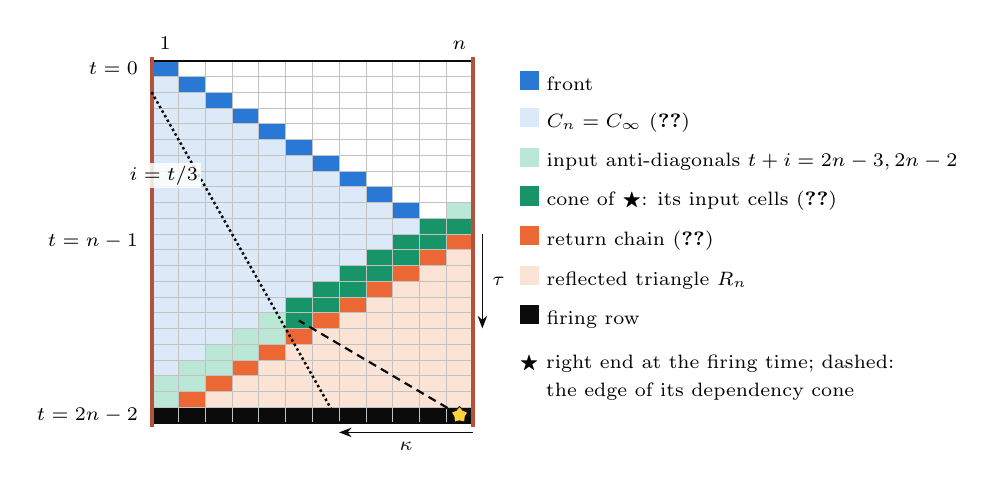
\begin{tikzpicture}[scale=1]
  \def\u{0.34}\def\v{0.2}
  \def\n{12}
  \pgfmathtruncatemacro{\T}{2*\n-2}
  \foreach \t in {0,...,\T} {%
    \foreach \i in {1,...,\n} {%
      \pgfmathtruncatemacro{\s}{\t+\i}
      \pgfmathtruncatemacro{\lc}{\i-1}
      \pgfmathtruncatemacro{\kap}{\n-\i}
      % default: quiescent
      \def\cc{white}
      \ifnum\t>\lc \def\cc{agree}\fi
      \ifnum\t=\lc \def\cc{stG}\fi
      \ifnum\s>20
        % the two input anti-diagonals t+i = 21, 22
        \ifnum\s<23
          \def\cc{stB!30}%
          \ifnum\kap<7
            \ifnum\s=22 \def\cc{stB!85!black}\fi
            \ifnum\s=21 \ifnum\kap>0 \def\cc{stB!85!black}\fi\fi
          \fi
        \fi
      \fi
      \ifnum\s=23 \def\cc{stA}\fi
      \ifnum\s>23 \def\cc{refl}\fi
      \ifnum\t=\T \def\cc{stF}\fi
      \filldraw[fill=\cc,draw=ink2!35,line width=0.2pt]
        (\i*\u-\u,-\t*\v) rectangle (\i*\u,-\t*\v-\v);
    }}
  \draw[ink,line width=0.6pt] (0,0) rectangle (\n*\u,-\T*\v-\v);
  % borders
  \draw[brick,line width=1.4pt] (0,0.05) -- (0,-\T*\v-\v-0.05);
  \draw[brick,line width=1.4pt] (\n*\u,0.05) -- (\n*\u,-\T*\v-\v-0.05);
  % backward dependency cone of the right end at the firing time
  \draw[ink,densely dashed,line width=0.8pt]
    (\n*\u-0.5*\u,-\T*\v-0.5*\v) -- (5.5*\u,-16.5*\v);
  \node[star,star points=5,fill=flash,draw=ink,line width=0.3pt,inner sep=0pt,
        minimum size=0.22cm] at (\n*\u-0.5*\u,-\T*\v-0.5*\v) {};
  % the line i = t/3
  % cell (t,i) has its centre at ((i-1/2)u, -(t+1/2)v); the line i = t/3
  \draw[ink,densely dotted,line width=0.9pt] (0,-2*\v) -- (7*\u,-23*\v);
  \node[font=\scriptsize,anchor=east,fill=white,fill opacity=0.85,text opacity=1,inner sep=1pt]
    at (1.85*\u,-7.3*\v) {$i=t/3$};
  % relative coordinates at the right end
  \draw[-{Stealth[length=1.6mm]},ink,line width=0.6pt]
    (\n*\u+0.12,-11*\v) -- node[right,font=\scriptsize] {$\tau$} (\n*\u+0.12,-17*\v);
  \draw[-{Stealth[length=1.6mm]},ink,line width=0.6pt]
    (\n*\u,-\T*\v-\v-0.12) -- node[below,font=\scriptsize] {$\kappa$} (\n*\u-5*\u,-\T*\v-\v-0.12);
  \node[font=\scriptsize,anchor=east] at (-0.05,-0.5*\v) {$t=0$};
  \node[font=\scriptsize,anchor=east] at (-0.05,-11.5*\v) {$t=n-1$};
  \node[font=\scriptsize,anchor=east] at (-0.05,-22.5*\v) {$t=2n-2$};
  \node[font=\scriptsize,anchor=south] at (0.5*\u,0.02) {$1$};
  \node[font=\scriptsize,anchor=south] at (\n*\u-0.5*\u,0.02) {$n$};
  % legend
  \begin{scope}[font=\scriptsize,align=left]
    \node[anchor=west] at (4.55,-0.25) {\textcolor{stG}{\rule{7pt}{7pt}} front};
    \node[anchor=west] at (4.55,-0.75) {\textcolor{agree}{\rule{7pt}{7pt}} $C_n=C_\infty$ (\cref{lem:agree})};
    \node[anchor=west] at (4.55,-1.25) {\textcolor{stB!30}{\rule{7pt}{7pt}} input anti-diagonals $t+i=2n-3,2n-2$};
    \node[anchor=west] at (4.55,-1.75) {\textcolor{stB!85!black}{\rule{7pt}{7pt}} cone of $\bigstar$: its input cells (\cref{lem:cone})};
    \node[anchor=west] at (4.55,-2.25) {\textcolor{stA}{\rule{7pt}{7pt}} return chain (\cref{lem:return})};
    \node[anchor=west] at (4.55,-2.75) {\textcolor{refl}{\rule{7pt}{7pt}} reflected triangle $R_n$};
    \node[anchor=west] at (4.55,-3.25) {\textcolor{stF}{\rule{7pt}{7pt}} firing row};
    \node[anchor=west] at (4.55,-3.85) {$\bigstar$ right end at the firing time; dashed:};
    \node[anchor=west] at (4.55,-4.2) {\phantom{$\bigstar$ }the edge of its dependency cone};
  \end{scope}
\end{tikzpicture}
}
\caption{The line of length $n=12$ (time downwards; colours show regions, not
states). $R_n$ is computed from the two input anti-diagonals
(\cref{lem:determinacy}); the firing of the right end ($\bigstar$) depends only
on the dark input cells (\cref{lem:cone}), which end where the line $i=t/3$
crosses the input anti-diagonals (\cref{thm:third}).}
\label{fig:anatomy}
\end{figure}

\begin{lemma}[pumping]\label{lem:pumping}
Let $2\le n<n'$ and let $\delta$ synchronize the lines of lengths $n$ and $n'$
at times $2n-2$ and $2n'-2$. Then $J_n$ and $J_{n'}$ differ on
$\mathrm{cone}_n(n-1,0)$.
\end{lemma}

\begin{proof}
Otherwise, by \cref{lem:determinacy,lem:cone}, the relative cell $(n-1,0)$ of
$R_{n'}$ (it lies in $R_{n'}$, and its cone has the same positions, away from
the left border $\kappa=n'$) has the value of the relative cell $(n-1,0)$ of
$R_n$, namely $C_n(2n-2,n)=\mathsf F$. Thus $C_{n'}(n'+n-2,n')=\mathsf F$
although $n'+n-2<2n'-2$.
\end{proof}

We write $\mathrm{PUMP}(n,n')$ for the conclusion of \cref{lem:pumping}; it is
a condition on $C_\infty$ alone. In the frame of the front,
$\Phi_t(j):=C_\infty(t,t+1-j)$ for $0\le j\le t$ is the cell at \emph{depth} $j$
behind the front, and the recurrence becomes
\begin{equation}\label{eq:comoving}
\Phi_{t+1}(j)=\delta\bigl(\Phi_t(j),\,\Phi_t(j-1),\,\Phi_t(j-2)\bigr)
\qquad(0\le j\le t+1),
\end{equation}
with $\Phi_t(-1)=\Phi_t(-2)=\mathsf L$ and $\Phi_t(t+1)=\ast$: information only
travels to larger depths, and the \emph{depth-row} $t\mapsto\Phi_t(j)$ starts
at time $j$. In these coordinates
$J_n(\kappa)=(\Phi_{n-3+\kappa}(2\kappa-2),\Phi_{n-2+\kappa}(2\kappa-1))$.

\begin{theorem}[speed-$1/3$ barrier]\label{thm:third}
Let $\delta$ be a minimal-time solution. Every depth-row $t\mapsto\Phi_t(j)$ is
eventually periodic; let $\theta(j)$ be the least $t_0\ge j$ such that it is
periodic on $[t_0,\infty)$. For every $n\ge4$ there is a depth $j\le n$ with
$\theta(j)>n+\tfrac{j}{2}-\tfrac52$. Hence
$\limsup_{j\to\infty}\theta(j)/j\ge 3/2$: along infinitely many depth-rows the
non-periodic part extends, up to an arbitrarily small angle, to the line
$i=t/3$.
\end{theorem}

\begin{proof}
Row $0$ satisfies $\Phi_{t+1}(0)=\delta(\Phi_t(0),\mathsf L,\mathsf L)$ and is
eventually periodic; by \eqref{eq:comoving}, row $j$ is a finite-state system
driven by the eventually periodic rows $j-1,j-2$, hence eventually periodic,
with some period $P_j$ (cf.\ \cite[\S4]{MazoyerTerrier94}). Fix $n\ge4$ and a
common multiple $P$ of $P_0,\dots,P_{n-1}$. The input cells of the cone at
$\kappa=0$ are quiescent in $R_n$ and $R_{n+P}$ (\cref{lem:lightcone}); the
others have depth $2\kappa-2$ (lower) or $2\kappa-1$ (upper), at most $n-1$ by
\cref{lem:cone}. If each of them lies in the periodic part of its row, i.e.\
$n-3+\kappa\ge\theta(2\kappa-2)$ for the lower and $n-2+\kappa\ge\theta(2\kappa-1)$
for the upper ones, then $J_{n+P}=J_n$ on the cone, contradicting
\cref{lem:pumping}. So some such cell, of depth $j\le n$, has
$\theta(j)>n-3+\kappa\ge n+\frac{j}{2}-\frac52$. If
$\limsup\theta(j)/j<3/2$, then $\theta(j)\le\alpha j+\beta$ for all $j$ with some
$\tfrac12\le\alpha<\tfrac32$ and $\beta$, and for $n$ large and all $j\le n$ we
get $(\alpha-\tfrac12)j\le(\alpha-\tfrac12)n<n-\beta-\tfrac52$, i.e.\
$\theta(j)\le n+\tfrac j2-\tfrac52$, a contradiction. Finally, the cell of depth
$j$ at time $\theta(j)$ is at position $\theta(j)+1-j$, which is at least
$\theta(j)/3+1$ when $\theta(j)\ge 3j/2$.
\end{proof}

\begin{remark}\label{rem:optimal}
The speed-$1/3$ signal of Waksman's and Balzer's constructions runs along the
line $i=t/3$; in Mazoyer's solution the periodic zone behind the front ends at
speed $1/2$ (observed up to time $2600$: $\theta(j)\in\{2j+1,2j+2\}$ for
$1\le j<700$, with period $3$). Computations suggest that the constant $3/2$ is
the best that \cref{lem:pumping} alone can give: on the half-line of the
five-state rule $\delta_{12}$ of \cref{sec:computations}, observed up to time
$1400$, $\theta(j)=\lceil 3j/2\rceil+2$ for $10\le j\le300$, with period $1$,
and the half-line satisfies $\mathrm{PUMP}(n,n')$ for all $4\le n<n'\le650$,
but it is excluded by the second barrier (\cref{cor:germ12}).
\end{remark}

%% ---------------------------------------------------------------------
\section{The left end: a second barrier}\label{sec:left}

Near the left border the reflected triangle is produced by a band of
anti-diagonals behind the reflected wave, which acts like a finite automaton
reading the half-line and must fire each cell exactly when it arrives there.
Put $v_c(i):=C_n(2n-2+c-i,\,i)$ for $c\ge0$ and $\max(1,c)\le i\le n$, and for
$c=-1$ and $1\le i\le n-1$: the cell of the \emph{chain} $t+i=2n-2+c$ at
position $i$. Chains $-1$ and $0$ are the input anti-diagonals and chain $1$ is
the return chain. The predecessors of $(2n-2+c-i,i)$ lie on the chains $c-2$,
$c-1$, $c$, so
\begin{equation}\label{eq:chains}
v_c(i)=\delta\bigl(v_{c-2}(i-1),\,v_{c-1}(i),\,v_c(i+1)\bigr)\qquad(c\ge1),
\end{equation}
with $v_{c-2}(0)$ and $v_c(n+1)$ standing for the border. If the line of length
$n$ is synchronized at time $2n-2$, then $v_i(i)=\mathsf F$ and
$v_c(i)\ne\mathsf F$ for $c<i$. In the skewed coordinates
$u_c(y):=v_c(y+\lfloor c/2\rfloor)$ this becomes
\begin{equation}\label{eq:slices}
u_c(y)=\delta\bigl(u_{c-2}(y),\,u_{c-1}(y+\varepsilon_c),\,u_c(y+1)\bigr),
\qquad \varepsilon_c=1\text{ for even }c,\ \varepsilon_c=0\text{ for odd }c,
\end{equation}
with $u_0(y)=C_\infty(2n-2-y,y)$ and $u_{-1}(y)=C_\infty(2n-2-y,y-1)$; here
$u_c(y)$ is the cell $y+\lfloor c/2\rfloor$ at time
$2n-2+\lceil c/2\rceil-y$, which is $\mathsf F$ if $\lceil c/2\rceil=y$ and not
$\mathsf F$ if $\lceil c/2\rceil<y$. Each slice $(u_1(y),u_2(y),\dots)$ is thus
computed from the slice $y+1$ and the input cells $u_{-1}(y),u_0(y)$
(\cref{fig:chains}). A word $w$ on an integer interval $I$ is
\emph{$\ell$-periodic} if $w(y+\ell)=w(y)$ whenever $y,y+\ell\in I$.

\begin{figure}[t]
\centering
\scalebox{0.92}{%% The lower left corner of the line of length n = 12: chains (anti-diagonals
%% t+i = 2n-2+c) and slices u(y) of the proof of the left-border lemma (s = 2).
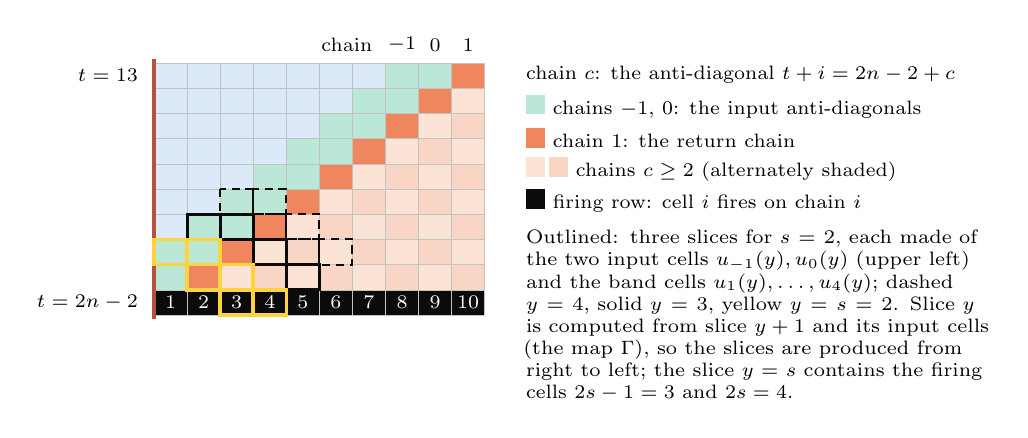
\begin{tikzpicture}[scale=1]
  \def\u{0.42}\def\v{0.32}
  \def\tz{13}   % first time shown
  % cell (t,i) occupies [(i-1)u, iu] x [-(t-tz+1)v, -(t-tz)v]
  \foreach \t in {13,...,22} {%
    \foreach \i in {1,...,10} {%
      \pgfmathtruncatemacro{\c}{\t+\i-22}
      \pgfmathtruncatemacro{\odd}{mod(\c+10,2)}
      \def\cc{agree}
      \ifnum\c>-2 \def\cc{stB!30}\fi
      \ifnum\c=1 \def\cc{stA!80}\fi
      \ifnum\c>1 \ifnum\odd=1 \def\cc{refl!60!stA!55}\else\def\cc{refl}\fi\fi
      \ifnum\t=22 \def\cc{stF}\fi
      \filldraw[fill=\cc,draw=ink2!35,line width=0.2pt]
        (\i*\u-\u,-\t*\v+\tz*\v) rectangle (\i*\u,-\t*\v+\tz*\v-\v);
    }}
  \draw[brick,line width=1.4pt] (0,0.05) -- (0,-10*\v-0.05);
  % outline of a cell: \cellbox{t}{i}{style}
  \def\cellbox#1#2#3{\draw[#3] (#2*\u-\u,-#1*\v+\tz*\v) rectangle (#2*\u,-#1*\v+\tz*\v-\v);}
  % slices y = 4 (dashed), 3 and 2 = s (solid); inputs u_{-1}, u_0 and band u_1..u_4
  \foreach \t/\i in {18/3,18/4,19/4,19/5,20/5,20/6} {\cellbox{\t}{\i}{ink,line width=0.7pt,densely dashed}}
  \foreach \t/\i in {19/2,19/3,20/3,20/4,21/4,21/5} {\cellbox{\t}{\i}{ink,line width=1.1pt}}
  \foreach \t/\i in {20/1,20/2,21/2,21/3,22/3,22/4} {\cellbox{\t}{\i}{flash,line width=1.3pt}}
  % chain numbers: on the firing row cell i lies on chain i
  \foreach \i in {1,...,10} {\node[font=\scriptsize,text=white] at (\i*\u-0.5*\u,-9.5*\v) {\i};}
  % chains -1, 0, 1 cross the first row shown at the cells 8, 9, 10
  \node[font=\scriptsize,anchor=south] at (7.5*\u,0.02) {$-1$};
  \node[font=\scriptsize,anchor=south] at (8.5*\u,0.02) {$0$};
  \node[font=\scriptsize,anchor=south] at (9.5*\u,0.02) {$1$};
  \node[font=\scriptsize,anchor=south east] at (6.9*\u,0.02) {chain};
  \node[font=\scriptsize,anchor=east] at (-0.08,-9.5*\v) {$t=2n-2$};
  \node[font=\scriptsize,anchor=east] at (-0.08,-0.5*\v) {$t=13$};
  % legend
  \begin{scope}[font=\scriptsize,align=left]
    \node[anchor=west] at (4.6,-0.15) {chain $c$: the anti-diagonal $t+i=2n-2+c$};
    \node[anchor=west] at (4.6,-0.55) {\textcolor{stB!30}{\rule{7pt}{7pt}} chains $-1$, $0$: the input anti-diagonals};
    \node[anchor=west] at (4.6,-0.95) {\textcolor{stA!80}{\rule{7pt}{7pt}} chain $1$: the return chain};
    \node[anchor=west] at (4.6,-1.35) {\textcolor{refl}{\rule{7pt}{7pt}}\,\textcolor{refl!60!stA!55}{\rule{7pt}{7pt}} chains $c\ge2$ (alternately shaded)};
    \node[anchor=west] at (4.6,-1.75) {\textcolor{stF}{\rule{7pt}{7pt}} firing row: cell $i$ fires on chain $i$};
    \node[anchor=north west,text width=5.9cm] at (4.6,-2.0) {Outlined: three slices for $s=2$, each made
      of the two input cells $u_{-1}(y),u_0(y)$ (upper left) and the band cells $u_1(y),\dots,u_4(y)$;
      dashed $y=4$, solid $y=3$, yellow $y=s=2$. Slice $y$ is computed from slice $y+1$ and its
      input cells (the map $\Gamma$), so the slices are produced from right to left; the slice $y=s$
      contains the firing cells $2s-1=3$ and $2s=4$.};
  \end{scope}
\end{tikzpicture}
}
\caption{The lower left corner of the line of length $n=12$ (time downwards;
colours show regions, not states). Outlined: three slices for $s=2$ (dashed
$y=4$, solid $y=3$, yellow $y=s$), each made of the input cells
$u_{-1}(y),u_0(y)$ (upper left) and the band cells $u_1(y),\dots,u_4(y)$; slice
$y$ is computed from slice $y+1$ (the map $\Gamma$ in the proof of
\cref{lem:left}), and slice $s$ contains the firing cells $2s-1$ and $2s$.}
\label{fig:chains}
\end{figure}

\begin{lemma}[left border]\label{lem:left}
Let $\delta$ have $k$ states and synchronize the line of length $n$ at time
$2n-2$. Let $s,\ell\ge1$ and $s\le Y\le n-s$, and suppose that the words
$y\mapsto C_\infty(2n-2-y,y)$ $(s\le y\le Y)$ and $y\mapsto C_\infty(2n-3-y,y)$
$(s\le y\le Y-1)$ are $\ell$-periodic. Then $Y-s\le(k-1)^{2s}\ell$.
\end{lemma}

\begin{proof}
For $s\le y\le Y$ let $\mathbf u(y):=(u_1(y),\dots,u_{2s}(y))$; these are cells
$y+\lfloor c/2\rfloor\le n$ with $\lceil c/2\rceil\le s\le y$, so they are
defined, and none is $\mathsf F$ when $y>s$. By \eqref{eq:slices}, $u_c(y)$,
$1\le c\le 2s$, is computed from components of index $<c$ of $\mathbf u(y)$, of
index $\le c$ of $\mathbf u(y+1)$, and from $u_{-1}(y),u_0(y)$; hence
$\mathbf u(y)=\Gamma(\mathbf u(y+1),u_{-1}(y),u_0(y))$ for $s+1\le y\le Y-1$,
with $\Gamma$ depending on $\delta$ only. Unfolding \eqref{eq:slices} for even
$c$, $u_{2j}(y)=\delta(u_{2j-2}(y),u_{2j-1}(y+1),u_{2j}(y+1))$, shows that
$u_{2s}(y)=\Gamma'(\mathbf u(y+1),u_0(y))$ for $s\le y\le Y-1$. By hypothesis,
$u_0$ is $\ell$-periodic on $[s,Y]$ and $u_{-1}$ on $[s+1,Y]$.

Suppose $Y-s>(k-1)^{2s}\ell$. The pairs $(\mathbf u(y),y\bmod\ell)$,
$s+1\le y\le Y$, take at most $(k-1)^{2s}\ell$ values, so there are
$s+1\le y_1<y_2\le Y$ with $\mathbf u(y_1)=\mathbf u(y_2)$ and $\ell\mid
h:=y_2-y_1$. By downward induction, $\mathbf u(y)=\mathbf u(y+h)$ for
$s+1\le y\le y_1$: if it holds for $y+1\le y_1$, then $\mathbf
u(y)=\Gamma(\mathbf u(y+1),u_{-1}(y),u_0(y))=\Gamma(\mathbf
u(y+1+h),u_{-1}(y+h),u_0(y+h))=\mathbf u(y+h)$, as $y+h<y_2\le Y$. Since
$s+h\le Y-1$ and $u_0(s+h)=u_0(s)$,
\[
u_{2s}(s+h)=\Gamma'(\mathbf u(s+1+h),u_0(s+h))=\Gamma'(\mathbf u(s+1),u_0(s))=u_{2s}(s)=\mathsf F,
\]
although $\lceil 2s/2\rceil=s<s+h$, so that $u_{2s}(s+h)$, the cell $2s+h$ at
time $2n-2-h$, is not $\mathsf F$: a contradiction.
\end{proof}

\begin{theorem}[left-border barrier]\label{thm:left}
Let $\delta$ be a minimal-time solution. There are no $s\ge1$, $\alpha>0$, $t_0$
and $p,q\ge1$ such that $C_\infty(t+p,i)=C_\infty(t,i)$ and
$C_\infty(t,i+q)=C_\infty(t,i)$ whenever the cells involved lie in the wedge
$\Omega:=\{(t,i):\ s\le i\le\alpha t,\ t\ge t_0\}$.
\end{theorem}

\begin{proof}
Suppose otherwise and put $\ell:=pq$. If $(t,i)$ and $(t-\ell,i+\ell)$ lie in
$\Omega$, so do the cells $(t-\ell,i+jq)$, $0\le j\le p$, and
$(t-\ell+jp,i)$, $0\le j\le q$, hence
$C_\infty(t-\ell,i+\ell)=C_\infty(t-\ell,i)=C_\infty(t,i)$. Let
$Y_n:=\lfloor\alpha(2n-3)/(1+\alpha)\rfloor$. For $s\le y\le Y_n$ the cells
$(2n-2-y,y)$ and $(2n-3-y,y)$ satisfy $y\le\alpha(2n-3-y)$, so they lie in
$\Omega$ once $2n-3-Y_n\ge t_0$, i.e.\ for $n$ large; since a step of $\ell$
positions along an anti-diagonal is the step from $(t,i)$ to
$(t-\ell,i+\ell)$, the words of \cref{lem:left} are $\ell$-periodic on
$[s,Y_n]$ and $[s,Y_n-1]$. As $Y_n\ge\frac{2\alpha}{1+\alpha}n-4$, for $n$ large
$Y:=\min(Y_n,n-s)$ satisfies $Y-s>(k-1)^{2s}\ell$, contradicting
\cref{lem:left}.
\end{proof}

The half-line of a rule is \emph{eventually regular} if there are $t_1$,
$P\ge1$ and, for each residue $r\in\{0,\dots,P-1\}$, an integer $m$, words
$w_0,\dots,w_m$, nonempty words $z_1,\dots,z_m$ over $W$ and integers
$a_j,D_j\ge0$ (all depending on $r$) such that for all $\nu\ge0$ the
configuration $C_\infty(t,1)\cdots C_\infty(t,t+1)$ at time $t=t_1+r+\nu P$ is
$w_0z_1^{a_1+\nu D_1}w_1\cdots z_m^{a_m+\nu D_m}w_m$: finitely many periodic
regions separated by signals of rational speeds.

\begin{corollary}\label{cor:regular}
The half-line of a minimal-time solution is not eventually regular.
\end{corollary}

\begin{proof}
Suppose it is. For each residue $r$ some $D_j$ is positive, because the
configuration grows by $P$ cells per period; let $j(r)$ be the least such
index. The blocks and junctions left of $z_{j(r)}$ have constant lengths, so
the block $z_{j(r)}^{a_{j(r)}+\nu D_{j(r)}}$ starts at a fixed cell $s_r$ and its
length grows at least like $\beta t$, for some $\beta>0$ and $t$ large. Inside
it the state of a cell depends only on its distance to $s_r$ modulo
$|z_{j(r)}|$, and is the same at the times $t$ and $t+P$. With
$s:=\max_r s_r$, $q:=\prod_r|z_{j(r)}|$, $\alpha:=\beta/2$ and $t_0$ large, every
cell of $\{(t,i):s\le i\le\alpha t,\ t\ge t_0\}$ lies in the block of index
$j(r)$ of its residue class, so $C_\infty$ is periodic with periods $P$ in time
and $q$ in space on this wedge, contradicting \cref{thm:left}.
\end{proof}

\begin{remark}\label{rem:left}
The proof of \cref{lem:left} uses only \eqref{eq:chains} for $c\ge1$, the
firing condition and the periodicity of the chains $c=-1,0$. Applied to the
mirror image of the line, it shows: if $\delta$ synchronizes the line of length
$n$ at time $2n-2$, $s\le Y\le n-s$ and $Y-s>(k-1)^{2s}\ell$, then the words
$y\mapsto C_n(2n-2-y,n+1-y)$ $(s\le y\le Y)$ and $y\mapsto C_n(2n-3-y,n+1-y)$
$(s\le y\le Y-1)$ are not both $\ell$-periodic; for $2y<n$ these cells lie in
$R_n$. In the classical constructions the structure required by
\cref{thm:left} is the family of signals of speeds $1/(2^j-1)$ accumulating at
the border \cite{Waksman66,Balzer67}, or the recursive division points
\cite{Mazoyer87}.
\end{remark}

%% ---------------------------------------------------------------------
\section{Applications to four and five states}\label{sec:computations}

The CNF formula $\mathrm{MT}_k(\mathcal N;M,N')$ has one-hot variables for the
entries of a $k$-state rule table, for the cells of $C_\infty$ with
$t+i\le M$, and for the cells of $R_n$, $n\in\mathcal N$. Its clauses say that
these cells follow the rule, that no half-line cell fires
\eqref{eq:neverfire}, that the line of length $n\in\mathcal N$ fires at time
$2n-2$ and not before, and that the return chains of \cref{lem:return} differ
from $C_\infty$; they add $\mathrm{PUMP}(n,n')$ for $4\le n<n'\le N'$
($\mathrm{MT}_k(\mathcal N;M)$ has none). All families follow from the
definition of minimality and the lemmas above, so the formula is satisfiable
if a $k$-state minimal-time solution exists. (An optional symmetry breaking,
by first occurrence of the auxiliary states in time-major order, is used by
none of the formulas below.) As a test, Mazoyer's solution, extracted
mechanically from Duprat's Coq development \cite{Duprat97} whose correctness
proof is described in \cite{Duprat02}, satisfies
$\mathrm{MT}_6(\{3,\dots,12\};78,40)$ (the extracted table synchronizes the
lengths $n\ge3$), and every model found by a solver was re-simulated by an
independent checker. All claims of this section are computer-assisted: the
unsatisfiability of each generated formula is certified by an LRAT proof
\cite{CruzFilipeEtAl17}, obtained from CaDiCaL \cite{CaDiCaL2} or from Kissat
\cite{Kissat20} via \textsf{drat-trim} and checked by \texttt{lrat-check}
\cite{WetzlerHeuleHunt14}, whereas the formula generator, the enumeration and
the simulations are trusted programs, tested as described.

\begin{theorem}\label{thm:four}
No four-state rule satisfying \eqref{eq:quiescence} synchronizes all lines of
lengths $2,\dots,9$ in minimal time; in particular no four-state minimal-time
solution exists.
\end{theorem}

\begin{proof}
Such a rule yields a model of $\mathrm{MT}_4(\{2,\dots,9\};16)$: a half-line
cell with $t+i\le16$ is quiescent if $i\ge10$ (\cref{lem:lightcone}) and equals
a cell of the line of length $9$ at a time $t<16$ if $i\le9$
(\cref{lem:agree}), so it does not fire, and the return chains hold by
\cref{lem:return} for $2\le n\le8$. CaDiCaL refutes this formula ($753$
variables, $17{,}605$ clauses, SHA-256
\texttt{d18d65480e77505193b8f60362badad5}\allowbreak\texttt{e71f8f08505f29befbcd3b2b18cdaabf})
in $51$\,s with an LRAT proof of $177$\,MB, which \texttt{lrat-check} verifies
in $5.7$\,s.
\end{proof}

The bound $9$ is sharp: an exhaustive enumeration finds $27$ partial rules
(rules restricted to the transitions they use) for the lengths $2,\dots,8$.
Yun\`es \cite{Yunes93}, who also imposes $\delta(\ast,\mathsf L,\mathsf
L)=\mathsf L$, found $27$ as well; none of ours uses $(\ast,\mathsf L,\mathsf
L)$. Sanders' example rule for the lengths up to $8$ \cite{Sanders94} is one of
them.

\paragraph{The five-state frontier} A five-state table has $94$ free entries
with five values, against $43$ entries with four values for four states.

\begin{proposition}\label{prop:chaotic}
The five-state rule $\delta_{14}$ of \cref{tab:delta14} synchronizes the line
of length $n$ at time $2n-2$ for every $2\le n\le14$; on the line of length
$15$ the cells $13,14,15$ fire at time $22$. Its half-line uses $16$
neighbourhoods besides $(\mathsf L,\mathsf L,\mathsf L)$ on the cells with
$t+i\le10^4$, none of them firing, and satisfies $\mathrm{PUMP}(n,n')$ for
$4\le n<n'\le800$; for $n\le5000$, $s\le3$ and $\ell\le24$, \cref{lem:left}
does not apply to its input anti-diagonals.
\end{proposition}

\begin{proof}
Direct simulation, by programs independent of the encoder.
\end{proof}

\begin{table}[t]
\centering\small
\setlength{\tabcolsep}{4pt}
\begin{tabular}{@{}cc|ccccc@{\hspace{1.4em}}cc|ccccc@{}}
\toprule
$x$ & $y$ & $\ast$ & $\mathsf L$ & $\mathsf G$ & $\mathsf A$ & $\mathsf B$ &
$x$ & $y$ & $\ast$ & $\mathsf L$ & $\mathsf G$ & $\mathsf A$ & $\mathsf B$\\
\midrule
$\ast$ & $\mathsf L$ & -- & $\mathsf F$ & $\mathsf F$ & $\mathsf L$ & $\mathsf G$ &
$\ast$ & $\mathsf A$ & -- & $\mathsf G$ & $\mathsf G$ & $\mathsf L$ & $\mathsf G$\\
$\mathsf L$ & $\mathsf L$ & $\mathsf L$ & $\mathsf L$ & $\mathsf G$ & $\mathsf G$ & $\mathsf B$ &
$\mathsf L$ & $\mathsf A$ & $\mathsf A$ & $\mathsf B$ & $\mathsf G$ & $\mathsf B$ & $\mathsf A$\\
$\mathsf G$ & $\mathsf L$ & $\mathsf G$ & $\mathsf A$ & $\mathsf B$ & $\mathsf A$ & $\mathsf B$ &
$\mathsf G$ & $\mathsf A$ & $\mathsf B$ & $\mathsf A$ & $\mathsf G$ & $\mathsf L$ & $\mathsf A$\\
$\mathsf A$ & $\mathsf L$ & $\mathsf G$ & $\mathsf B$ & $\mathsf G$ & $\mathsf G$ & $\mathsf G$ &
$\mathsf A$ & $\mathsf A$ & $\mathsf B$ & $\mathsf L$ & $\mathsf A$ & $\mathsf G$ & $\mathsf A$\\
$\mathsf B$ & $\mathsf L$ & $\mathsf A$ & $\mathsf B$ & $\mathsf A$ & $\mathsf A$ & $\mathsf L$ &
$\mathsf B$ & $\mathsf A$ & $\mathsf L$ & $\mathsf A$ & $\mathsf A$ & $\mathsf G$ & $\mathsf A$\\
\midrule
$\ast$ & $\mathsf G$ & -- & $\mathsf L$ & $\mathsf F$ & $\mathsf L$ & $\mathsf L$ &
$\ast$ & $\mathsf B$ & -- & $\mathsf G$ & $\mathsf G$ & $\mathsf G$ & $\mathsf G$\\
$\mathsf L$ & $\mathsf G$ & $\mathsf F$ & $\mathsf A$ & $\mathsf F$ & $\mathsf B$ & $\mathsf A$ &
$\mathsf L$ & $\mathsf B$ & $\mathsf G$ & $\mathsf B$ & $\mathsf G$ & $\mathsf A$ & $\mathsf L$\\
$\mathsf G$ & $\mathsf G$ & $\mathsf B$ & $\mathsf B$ & $\mathsf F$ & $\mathsf G$ & $\mathsf F$ &
$\mathsf G$ & $\mathsf B$ & $\mathsf F$ & $\mathsf B$ & $\mathsf A$ & $\mathsf B$ & $\mathsf B$\\
$\mathsf A$ & $\mathsf G$ & $\mathsf B$ & $\mathsf A$ & $\mathsf G$ & $\mathsf G$ & $\mathsf A$ &
$\mathsf A$ & $\mathsf B$ & $\mathsf G$ & $\mathsf B$ & $\mathsf B$ & $\mathsf G$ & $\mathsf B$\\
$\mathsf B$ & $\mathsf G$ & $\mathsf B$ & $\mathsf A$ & $\mathsf G$ & $\mathsf A$ & $\mathsf L$ &
$\mathsf B$ & $\mathsf B$ & $\mathsf A$ & $\mathsf L$ & $\mathsf A$ & $\mathsf A$ & $\mathsf L$\\
\bottomrule
\end{tabular}
\caption{The rule $\delta_{14}$ of \cref{prop:chaotic}: the entry in row $(x,y)$
and column $z$ is $\delta(x,y,z)$; ``--'' marks the unused neighbourhoods
$(\ast,y,\ast)$. Machine-readable copy: \texttt{results/delta14.txt} in the
repository.}
\label{tab:delta14}
\end{table}

For $3\le t<1500$ the half-line of $\delta_{14}$ takes the values
$\mathsf L,\mathsf G$ at cell $1$, $\mathsf L,\mathsf A$ at cell $2$ and
$\mathsf L,\mathsf B$ at the cells $i\ge3$; the rule restricted to $\{\mathsf
L,\mathsf B\}^3$ is the elementary cellular automaton rule $22$
\cite{Wolfram83}, so the half-line is rule $22$ driven at its left end by the
cells $1$ and $2$, and it is irregular. Four further rules, on three other
half-lines (up to renaming of states), also synchronize all lengths up to $14$
and fail at $15$. Hence
$\mathrm{MT}_5(\{2,\dots,14\};78,40)$ is satisfiable, neither barrier excludes
$\delta_{14}$ in the ranges of \cref{prop:chaotic}, and refutations along
these lines need lines of length at least $15$.

The left-border lemma does refute a more regular architecture. The rules
$\delta_{12}$ and $\delta_{13}$ (files \path{results/uniformA_2-12.txt} and
\path{results/delta13.txt}) synchronize every line of length at most $12$,
resp.\ $13$. Their half-lines coincide for $t+i\le78$, where they use the $22$
transitions
\begin{center}\small
\texttt{*GL>A GLL>G *AG>B AGL>L *BL>A BLG>L LGL>B *AL>G ALB>A LBG>L BGL>G}\\
\texttt{*GA>A GAL>L ALG>B LGG>G GGL>G BGG>L GGG>G ALL>A LLG>L ALA>A LAL>L}
\end{center}
(where \texttt{xyz>d} means $\delta(x,y,z)=d$) besides
$\delta(\mathsf L,\mathsf L,\mathsf L)=\mathsf L$, and consist of a front and a
wake of $\mathsf G$'s and, behind a boundary of speed $1/3$, a region
$\mathsf A\,\mathsf L\,\mathsf A\,\mathsf L\cdots$ periodic in time and space
(\cref{rem:optimal}).

\begin{corollary}\label{cor:germ12}
No five-state rule with the $22$ transitions above synchronizes the line of
length $518$ in minimal time.
\end{corollary}

\begin{proof}
With these transitions and $\delta(\mathsf L,\mathsf L,\mathsf L)=\mathsf L$
only, no other neighbourhood occurs on the cells with $t+i\le1034$, so every
such rule has the same diagram $C_\infty$ there. On $t+i=1034$ the cells
$2,\dots,259$ are in state $\mathsf A$, and on $t+i=1033$ the cells
$2,\dots,258$ are in state $\mathsf L$. \Cref{lem:left} with $k=5$, $n=518$,
$s=2$, $\ell=1$, $Y=259$ would give $257\le4^4=256$.
\end{proof}

\paragraph{Half-lines of low complexity} The \emph{germ} below $M$ of a rule is
its restriction to the neighbourhoods of the cells $(t,i)$, $t\ge1$, $t+i\le M$,
of its half-line, and its \emph{complexity} $c_M(\delta)$ is the number of these
neighbourhoods other than $(\mathsf L,\mathsf L,\mathsf L)$: $c_{78}=57$ for
Mazoyer's rule, $22$ for $\delta_{12}$ and $16$ for $\delta_{14}$.

\begin{proposition}\label{prop:germs}
Every five-state minimal-time solution $\delta$ satisfies $c_{78}(\delta)\ge15$.
\end{proposition}

\begin{proof}[Proof (computer-assisted; the SAT part is LRAT-certified)]
Suppose $c_{78}(\delta)\le14$. After exchanging $\mathsf A$ and $\mathsf B$ if
necessary, $\mathsf A$ occurs before $\mathsf B$ (if at all) when the cells are
ordered by anti-diagonal and, within an anti-diagonal, by time. By
\eqref{eq:neverfire} and \cref{lem:return,lem:pumping}, the germ of $\delta$
below $78$ produces no firing cell, never produces $\mathsf L$ at the front,
and satisfies $\mathrm{PUMP}(n,n')$ for $4\le n<n'\le40$. A depth-first search
that chooses the value of a neighbourhood when it first occurs enumerates all
such germs ($1.0\cdot10^8$ nodes): there are $244$, and an independent
re-implementation finds the same $244$. For $230$ of them,
$\mathrm{MT}_5(\{2,\dots,10\};78,39)$ (without symmetry breaking) together
with the germ is unsatisfiable: one formula with a selector variable per germ,
clauses that make each selector fix the transitions of its germ, and a clause
requiring some selector, is refuted by CaDiCaL in $4$\,s with an LRAT proof of
$11$\,MB. Each of the other $14$ germs determines $C_\infty$ up to the
anti-diagonal $3300$, and on these diagrams \cref{lem:left} applies with
$s=1$: there are $n\le163$ and $\ell\le5$ such that, for the line of length
$n$, the upper input anti-diagonal is $\ell$-periodic on $[1,Y]$ and the lower
one on $[1,Y-1]$ with $Y-1>16\ell$ (e.g.\ $n=28$, $\ell=1$, $Y=19$), as an
independent simulation confirms. Hence no rule containing one of the $244$
germs, in particular $\delta$, is a minimal-time solution.
\end{proof}

\paragraph{Balzer's conditions} Balzer \cite[p.~37]{Balzer67} reported that no
five-state minimal-time solution satisfies the four conditions
(B1) $\delta(x,\mathsf G,y)=\mathsf G$ unless $x,y\in\{\mathsf G,\ast\}$;
(B2) $\delta(I(z),I(y),I(x))=I(\delta(x,y,z))$ for an involution $I$ of the
states with $I(\ast)=\ast$ (an \emph{image solution});
(B3) $\delta(\mathsf G,\mathsf G,\mathsf G)=\delta(\ast,\mathsf G,\mathsf
G)=\delta(\mathsf G,\mathsf G,\ast)=\mathsf F$ and no other neighbourhood gives
$\mathsf F$;
(B4) $\delta(\mathsf G,v,\mathsf G)=\mathsf G$ for all $v\in W\setminus\{\mathsf
G\}$. His eight-state solution satisfies them, and Mazoyer's only (B3)
\cite{Mazoyer86Lyon}. In the \emph{weak reading} \cite{Yunes93}, (B1) is
required only for working states $x,y$ and (B3) without its last clause. We
take $I(\mathsf F)=\mathsf F$. Then $I(\mathsf G)=\mathsf G$ in both readings:
otherwise $g:=I(\mathsf G)\in W\setminus\{\mathsf G\}$, (B4) gives
$\delta(\mathsf G,g,\mathsf G)=\mathsf G$, hence $\delta(g,\mathsf G,g)=g$ by
(B2), whereas (B1) gives $\delta(g,\mathsf G,g)=\mathsf G$. So $I$ is one of the
four involutions of $\{\mathsf L,\mathsf A,\mathsf B\}$, and (B1)--(B4) become
unit and binary clauses.

\begin{proposition}\label{prop:balzer}
No five-state rule satisfying (B1)--(B4) in the weak reading, with $I(\mathsf
F)=\mathsf F$, synchronizes all lines of lengths $2,\dots,12$ in minimal time;
a fortiori none satisfying Balzer's (strong) form does. The lengths up to $11$
do not suffice to prove this.
\end{proposition}

\begin{proof}[Proof (computer-assisted; the SAT part is LRAT-certified)]
For each of the four involutions, the clauses of (B1)--(B4) in the weak reading
are added to $\mathrm{MT}_5(\{2,\dots,N\};2N-2)$, without symmetry breaking.
For $I=(\mathsf A\,\mathsf B)$ and $N=10$, and for $I=(\mathsf L\,\mathsf A)$
and $I=(\mathsf L\,\mathsf B)$ and $N=9$, CaDiCaL refutes the formula with LRAT
proofs checked in $7.1$, $3.5$ and $3.3$\,s. For $I$ the identity and $N=12$,
Kissat refutes it in $15$ minutes; \textsf{drat-trim} turns its DRAT proof into
an LRAT proof of $3.1$\,GB, which \texttt{lrat-check} verifies in $66$\,s. For
the last statement, the rule in \path{results/balzer_sym11.txt} satisfies
(B1)--(B4) in the strong, hence also in the weak, reading with $I$ the
identity, and it synchronizes every line of length at most $11$ (direct
simulation).
\end{proof}

With six states, for every type of involution there are rules satisfying
(B1)--(B4) in the strong reading that synchronize all lines of lengths up to
$13$, and for two types up to $14$, so a refutation of this kind would need longer lines; whether
Balzer's conditions exclude six states remains open.

%% ---------------------------------------------------------------------
\section{Concluding remarks}\label{sec:conclusion}

A minimal-time solution needs non-periodic structure reaching the line
$i=t/3$ and in every wedge at the left border; the known constructions provide
it with hierarchies of slow signals or division points, while the five-state
half-lines that survive our tests are irregular, and Lemma~\ref{lem:left} has no
grip on them in the ranges we checked. Natural questions are: (1) Does a
five-state minimal-time solution exist? A refutation along the lines of
\cref{thm:four} needs lines of length at least $15$. (2) Is there a necessary
condition like \cref{lem:pumping} on the reflected triangles themselves,
beyond \cref{rem:left}? (3) Can the bound $(k-1)^{2s}\ell$ of \cref{lem:left}
be made polynomial in $s$, or extended to anti-diagonals that are periodic up
to a bounded number of defects? (4) Do Balzer's conditions exclude six states?

\section*{Declarations}
\noindent\emph{CRediT.} All authors: Conceptualization, Methodology, Formal
analysis, Investigation, Validation, Writing -- review \& editing.
\emph{Competing interests.} None. \emph{Funding.} None. \emph{Data
availability.} Programs, formula generators, rule tables, logs, the SHA-256
digests of the formulas and certificates, and the commands that regenerate
the certificates and check every computational statement of this note are at
\url{https://github.com/giamkiakeng/proj1} (directory \texttt{fssp5}).
\emph{Use of generative AI.} The authors used Claude (Anthropic) to develop and
check the mathematical arguments, to write and run the programs, to carry out
the experiments and to draft and proofread the text; they reviewed and edited
the content and take full responsibility for it.

\renewcommand{\bibfont}{\small}
\bibliographystyle{elsarticle-num}
\bibliography{refs}

\end{document}
